\documentclass[11pt]{article}

\usepackage{fullpage}
\usepackage{xcolor}
\usepackage{amsmath}
\usepackage{graphicx}

\newcommand{\code}[1]{\mbox{\texttt{\textcolor{blue}{#1}}}}

\graphicspath{{./images/}}

\title{Assembler and Extension... }
\author{Vincent Ho, Kiky Chow, Jasper Liu, Julian Wong}

\begin{document}

\maketitle

\section{Introduction, Group Strategies and Reflections}

Having the experience from designing the emulator, we have learnt how to communicate with our groupmates effectively and come up a starting plan as soon as possible. We set deadlines for each individual parts and started the debugging process right after. In order to speed up our progress, some of us started with designing the extension at the same time while others continued with the debugging for the assembler. Like before, having regular meetings allowed us to keep updated with each other’s progress and was very helpful for seeking immediate help, which largely reduced our working time. It also made the debugging process very convenient as we could screen share and spot any errors quickly. Overall, our group has worked quite smoothly, but it may be even better if we could hold face-to-face meetings for future projects.\\

Furthermore, in this particular instance, for the sake of consistency in code, we decided to work on separate files for each part of the project and push to the master branch directly on Git every time. For a project of this scale, this meant that code clashes and merge conflicts could be kept to a minimum, and that each of us could write code that was dependent of other members' easier. However, we understand that in the future, creating remote branches for each member or for each section of a program would be the preferred strategy for a project of a larger scale.

\subsection{Vincent}

Working on a group programming project has not only allowed me to be more familiar with Git and C, but also enhanced my ability to find bugs and write better readable code in general. Given the circumstances of having to work collaboratively online, I have also learnt to communicate more clearly and to set deadlines earlier in case of any inconveniences. I have found that my group constantly maintains good communication and support especially when dealing with decisions on how the project should be implemented, allowing every single person to feel comfortable with each other throughout the project.\\

Going into this project initially, I thought that I would have a hard time compromising code style and management of files as everyone’s style is always different. However, I have learnt that communicating in advance about problems such as this vastly benefits and increases efficiency on my work, and I will definitely maintain this whilst working in future projects with different people. There are however several things I would do differently, but the main one is to ask for help when I feel stuck and ask about how someone implemented their function if I don’t understand instead of trying to figure it out myself. During the project, as I gradually asked more and communicated more with my group mates, I have found that my work efficiency has widely increased. In the future, I will seek for help or ask whenever I have something that I don’t quite understand. In general, I have felt that I have fitted in well in this group and I have learnt a lot from working on a project together.

\subsection{Kiky}

I think one of my weaknesses is to fully understand the specification without looking at code so at first I was a bit confused in the discussion of the implementation for the emulator. However, after I had started coding, I gain more insight into the problem and I am able to work ahead on the assembler and the extension while others are debugging the previous part. I am also stronger in writing functions than writing the main program. In the future, I would like to maintain the practice that we work in parallel. A groupmate can start working on the next part even the previous part had not passed all test cases so we do not put work close to the deadline.

\subsection{Jasper}

At first, I was a bit timid to ask for help when I had difficulties with my part of coding or with the understanding of the specification. However, after having frequent communication with my groupmates, I have learnt how to seek help or advices from them. Since I am not the best at debugging, I tried to help as much as I can with other parts like lab reports. In the future projects, I think I will communicate more with my groupmates in the next project and make sure everyone will seek help whenever they find helpful.

\subsection{Julian}

Programming amongst a team has definitely given me an insight into what software development is like in industry. I have gained invaluable experience in using Git within a team – how to avoid code conflicts and to keep my code up-to-date with others'. Furthermore, I have been able to experience coding distinct sections of a program and learn to ensure that these individual sections can behave properly, no matter if they are utility functions or data structures, so that other members of the team can confidently depend on my work and proceed with theirs. On another note, discussing and debating on abstract ideas like data structures and code implementation can often be difficult, especially when other members need to thoroughly understand your ideas and develop upon them, or point out their flaws. The patience, conciseness in words and clarity required to explain such concepts is definitely a skill that I need to grasp if I am to improve my performance in further projects and in industry.

\section{Assembler: Implementation and Structure}

We spread our work across the following files:

\begin{itemize}
\item \code{symbol\_table.c}: A representation of a table which stores labels and addresses
\item \code{tokenizer.c}: Splitting assembly instructions into their constituents
\item \code{transform.c}: Generating 32-bit instructions based on the constituents
\item \code{transform\_utils.c}: Contains additional helper functions for \code{transform.c}
\end{itemize}

We agreed on performing two passes across the assembly file when designing the assembler – the first of which stores any labels and their addresses into a \code{Symbol\_Table} struct, and the second generates 32-bit instructions whilst reading through the file line by line.\\

In \code{tokenizer.c}, we were able to separate a line of assembly code by using the \code{strtok\_r} and \code{strtol} functions, and store these constituents into the heap-allocated pointers \code{mnemonic}, \code{operands} and \code{expression}. In parallel with this process, we keep track of the current \code{pc\_addr} and the \code{end\_addr} of the assembly file by counting the line numbers.\\

In \code{transform.c}, we used the same strategy as we did in the emulator by splitting the main \code{assemble} function by instruction type and creating a sub-function for each type, e.g. \code{data\_processing\_to\_binary}, \code{branch\_to\_binary} etc., improving readability and removing duplicate code in the process. We reused some bit manipulation functions from the emulator, e.g. \code{get\_bits}, as well as the \code{mnemonic} and \code{suffix} enums so that we could get their corresponding opcodes more efficiently. Figure~\ref{fig:assembler_flow} shows how the additional variables, functions and \code{Symbol\_Table} struct contribute to the overall flow of the assembler.\\

\begin{figure}[h]
\centering
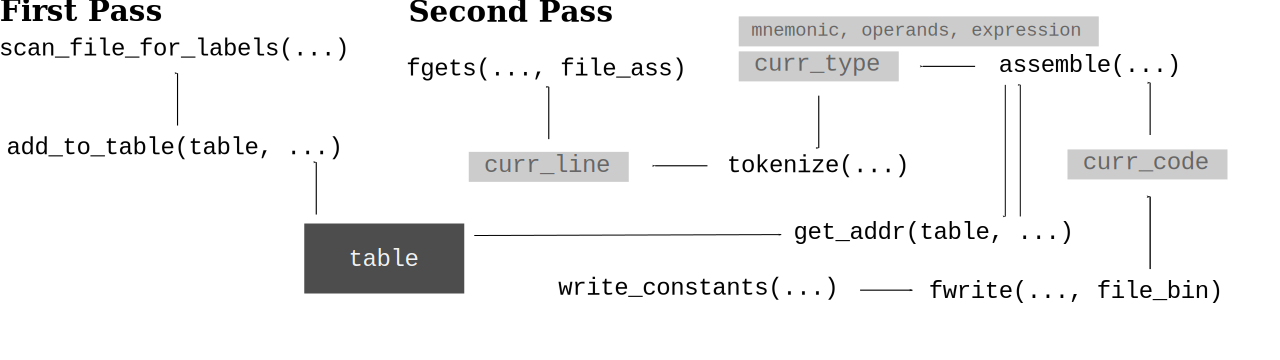
\includegraphics[width=\linewidth]{assembler_flow}
\caption{An illustration of the assembler's main functions and their dependencies}
\label{fig:assembler_flow}
\end{figure}

In the case of \code{ldr} instructions, we were able to store any constants larger than \code{0xFF} in the heap-allocated array \code{constants}. After the second pass, the constants are then written to the end of the binary file sequently using the \code{write\_constants} function.

\section{Introducing Our Extension – Evaluator}

After much discussion and design, we are proud to introduce the extension for our project – a formula evaluator for propositional logic. In other words, it is a high-level compiler which reads through a source file containing a logical formula, and generates the corresponding assembly file. By running this assembly file through the assembler and then the emulator, the truth value of this formula can be found in the register \code{\$0} of the ARM processor – 0 for false and 1 for true. In this source file, a \code{d} instruction declares a variable and assigns it with a truth value, whereas an \code{e} instruction tells the evaluator the formula that needs to be evaluated according to the truth values above. For example, the logical formula \(( \,p \Rightarrow q) \, \land ( \,p \Leftrightarrow q) \,\), with \(p\) and \(q\) being both \(\bot\), would be represented by the source file in Figure~\ref{fig:evaluator_sample_source}.

\begin{figure}[h]
\centering
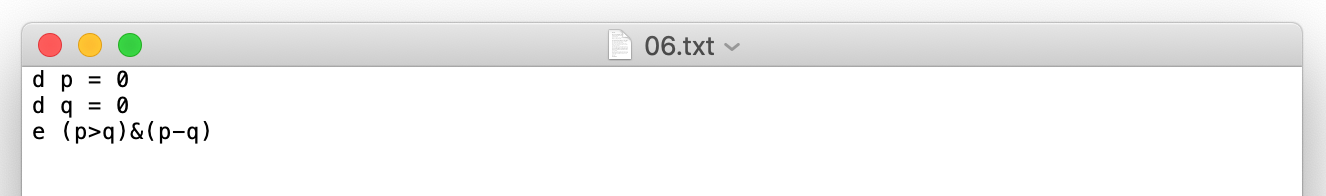
\includegraphics[width=\linewidth]{evaluator_sample_source}
\caption{An example of a source file for the evaluator}
\label{fig:evaluator_sample_source}
\end{figure}

For more information on what symbols are supported by our current evaluator, you can type \code{./evaluate help} when in the right folder, or view the \code{help.txt} file in our Git repository.\\

Using the above example, the evaluator would generate the assembly file in Figure~\ref{fig:evaluator_sample_assembly}. You can find more examples of source files and their compiled assembly and binary files in the \code{extension/testsuite/} folder.\\

\begin{figure}[h]
\centering
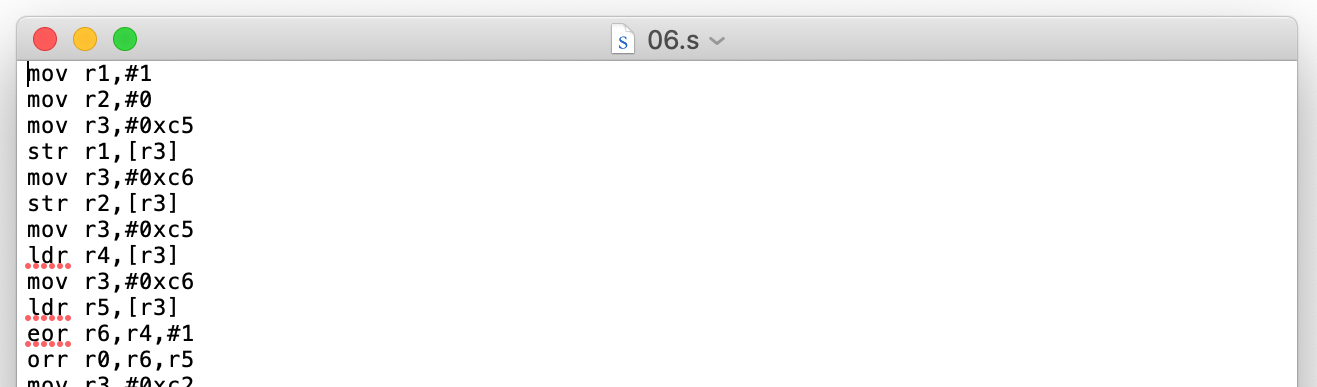
\includegraphics[width=\linewidth]{evaluator_sample_assembly}
\caption{An example of an assembly file compiled by the evaluator}
\label{fig:evaluator_sample_assembly}
\end{figure}

If you pass this assembly file into the assembler, and then the emulator, you will find that the \code{\$0} register in the output has a value of \code{1}, i.e. the original formula evaluates to \(\top\) given the truth values of \(p\) and \(q\).\\

\section{Evaluator: Implementation and Structure}

We spread our work across the following files:

\begin{itemize}
\item \code{evaluate.c}: Controlling the I/O of the evaluator
\item \code{parse\_tree.c}: Converting a string of formula into a parse tree
\item \code{assembly\_writer.c}: Converting a parse tree into assembly code
\end{itemize}

The evaluator first gets the variables, truth values and the formula from the source file through \code{decode\_source\_format(...)}, and stores them in a heap-allocated array of \code{Assignment}s and string variable respectively. It then passes the formula into the \code{to\_tree(...)} function, which generates a parse tree for the formula.\\

Finally, the tree, along with the \code{Assignment}s, are passed into the \code{write\_code(...)} function. In here, we traverse through the tree three times, almost like a three-pass process, in post-order. First, each variable node in the tree is assigned an `index' or `address' – note the \code{addr} attribute in the \code{Node} struct. Secondly, each variable node in the tree is assigned to its truth value via the \code{val} boolean attribute. Lastly, the tree is evaluated node by node through the \code{evaluate} function. Since all the operators are binary (with the exception of \code{NOT}), it is relatively straightforward to read a node (the operator) and its two children (the arguments), and thus generate the correct assembly code at each level of the tree.\\

Figure~\ref{fig:evaluator_tree_traversal} further illustrates how the processor / emulator can `traverse' through the parse tree (represented in memory) and assign each node a truth value when it is executing the resultant binary file.\\

\begin{figure}[h]
\centering
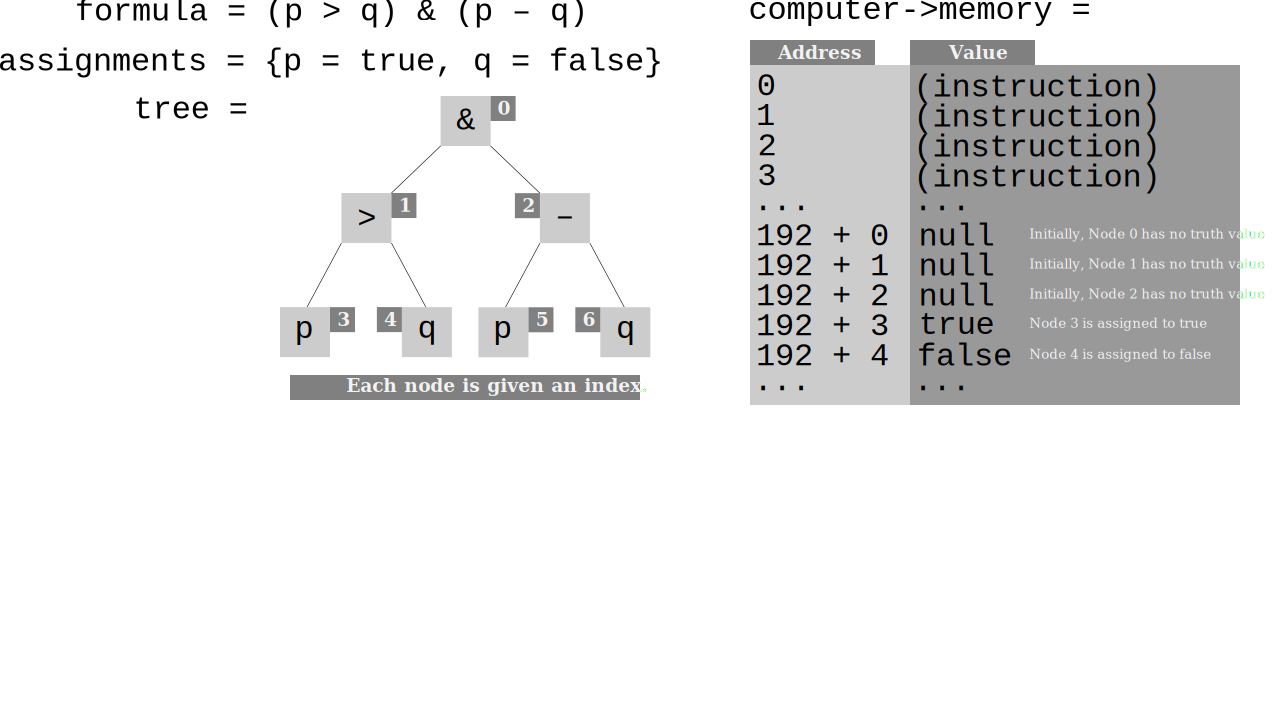
\includegraphics[width=\linewidth]{evaluator_tree_traversal}
\caption{An illustration of the tree traversal process in the evaluator}
\label{fig:evaluator_tree_traversal}
\end{figure}

The computer's memory in this example is at a state when all the variables have just been assigned to their truth values. In the next recursive call of \code{evaluate(...)}, Node 1 will be evaluated to \code{false}, since \(( \,p \Rightarrow q) \, \equiv \bot\). Therefore, the memory slot with the address \(192 + 1\) will be given the value \code{false}. This is so that when Node 0 is being evaluated, it can find its children (i.e. Node 1) by accessing memory address \(192 + 1\), and get the truth value of the subformula encompassed within Node 1, i.e. its entire sub-tree. This evaluation process was inspired by the Reverse Polish notation, and is relatively convenient to accomplish due to the binary nature of all the operators. In the case of the unary operator \code{NOT}, the right child of a \code{NOT} node will simply be null and will be ignored. The memory offset of 192 is to be explained in the next section.

\section{Evaluator: Design Challenges}

One of the main challenges when designing the evaluator was creating the parse tree structure. More specifically, we had to work out how to create a hierarchy for the logical operators depending on their binding strength, as well as dealing with brackets and subformulas within formulas. This explains why we needed a tree in the first place – due to the recursive nature of binary operators and brackets, but also the \code{operator} enum, which contains the relative binding strength of each operator (where \code{EMPTY} represents a primitive symbol, i.e. variable). Depending on the binding strength, we can then decide whether an operator needs to be `pushed' onto the top of the tree, or whether it can be added to the shallowest empty node. However, for the sake of efficiency in \code{assembly\_writer.c} later on, we have decided to deal with brackets separately (by recursively merging sub-trees into a main tree) rather than treating it as an operator.\\

Another major challenge was utilising the memory correctly during tree traversal. Originally, our plan was to pass the truth value of the evaluated subformula through recursion within the evaluator, and not by using memory spaces. However, the current implementation, though less kind and efficient towards the assembler and emulator, allows the emulator to execute the binary file in a way that is very similar to tree traversal, and is thus the more `realistic' approach. In order to allow space for the instructions of the assembly file \textit{and} the nodes' truth values to coexist, we have had to define a \code{MEMORY\_OFFSET} constant (currently arbitrarily set to 192). All the space below the address \code{MEMORY\_OFFSET} is allocated for the instructions, whereas the tree and its truth values live in the space above this address.

\section{Evaluator: Testing}

Due to the time constraints, we have yet been able to write a script to automate our testing process, but as you can see in our \code{extension/testsuite/} folder, we have created 6 pairs of test cases – 6 that should evaluate to \(\top\), and 6 that should evaluate to \(\bot\). The \code{cases\_output/} folder contains 12 `placeholder' files for the output of the evaluator and assembler – two for each pair of test cases. For the time being, we have run each \code{.txt} test case file through the evaluator and each resultant \code{.s} and \code{.bin} file across the assembler and emulator by hand. We have manually checked that the \code{\$0} register displays the correct result, and that the other registers and memory addresses store the correct values.\\

Our test cases range from formulae as simple as \(p \Rightarrow q\), to ones such as \(( \,p \land q) \, \lor ( \,p \lor q) \,\). In the process, we have covered every logical operator we support, as well as a diverse combination and arrangement of brackets. Additionally, the evaluator is able to detect when a formula, and thus its parse tree, is syntactically incorrect, and will assume that any undeclared variables evaluate to \(\bot\). As a result, the testing has been very comprehensive, and we believe that our evaluator will behave correctly for most, if not all, user inputs.

\end{document}
